\chapter{Implementación}

En este capítulo se detallará cómo se ha desarrollado la aplicación, comentando los desafíos y soluciones que han ido surgiendo a lo largo de este. Al usar un motor gráfico que \textbf{no usa código escrito convencional} y en su lugar usa un sistema de nodos conocido como Blueprint, el cual solo se puede visualizar a través del editor del motor, gran parte de este capítulo consistirá en mostrar estos Blueprints acompañados de sus respectivas explicaciones y diagramas de flujo. Estos últimos no coincidirán necesariamente uno a uno con sus respectivos Blueprints, ya que los diagramas se han diseñado para comprenderlos con mayor facilidad y por tanto combinan y ocultan elementos que, aunque deban estar dentro del Blueprint, no son necesarios para su explicación.

\section{Uso de Unreal Engine 5 y estructura del proyecto}

Al crear un proyecto de Unreal Engine, el motor crea de forma automática una estructura de carpetas con todo lo necesario para el funcionamiento del proyecto. La única relevante para este capítulo es la carpeta \textit{Content}, ya que es donde se encuentra todo el código y \textit{assets} creados para la aplicación. La carpeta \textit{Config} almacena datos de configuración varios del proyecto, y el resto son archivos compilados y de gestión varios que usa Unreal Engine para su funcionamiento. De hecho, no se incluyen en el repositorio de ChiselVR\footnote{\url{https://github.com/FINNO51/TFG_ChiselVR}} y han sido listados dentro del archivo \textit{.gitignore}.

Al iniciar el editor, se nos muestra la escena 3D, su árbol de la escena con todos los objetos añadidos y un navegador de archivos. Desde este último, se pueden crear nuevos objetos (Blueprints) para luego arrastrarlos a la escena y usarlos libremente (Figura \ref{fig:unrealinicio}).

\begin{figure}[H]
	\centering
	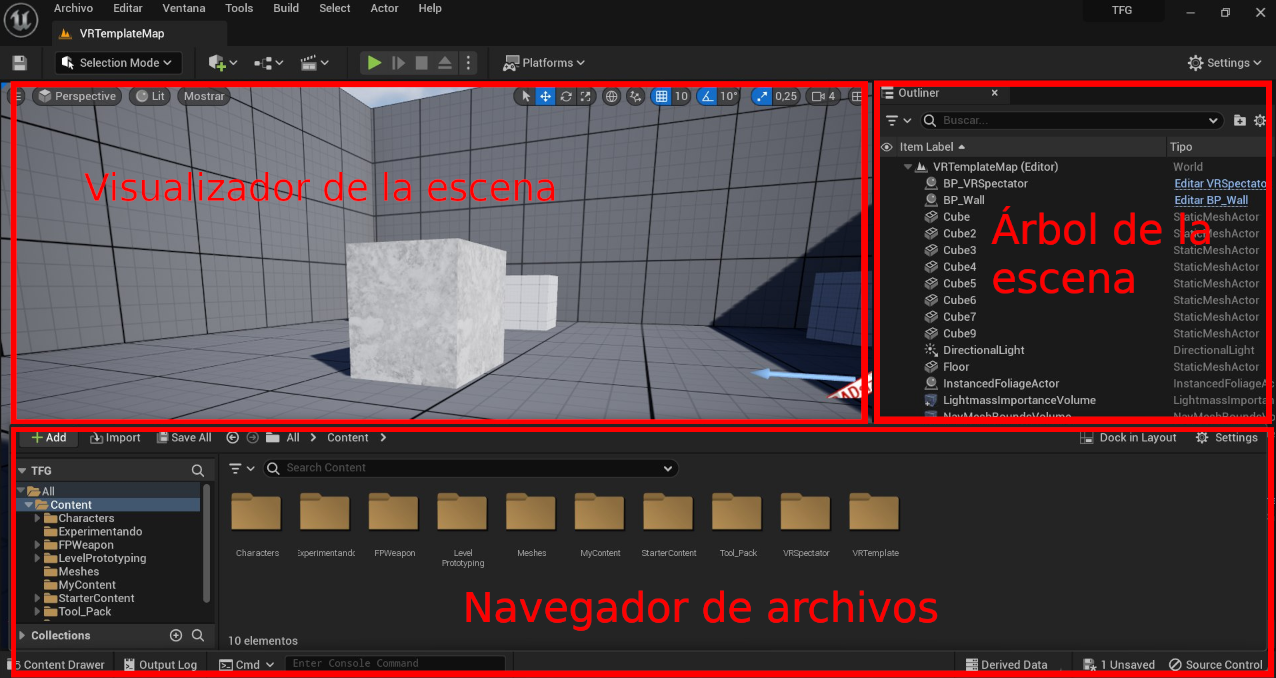
\includegraphics[width=10cm]{imagenes/unrealinicio}
	\caption{Editor de Unreal Engine 5.}
	\label{fig:unrealinicio}
\end{figure}

En el desarrollo de ChiselVR se han usado, aparte de distintos modelos 3D y efectos que se mencionarán a su debido tiempo, cuatro elementos principales: \texttt{BP\_Block} y \texttt{BP\_Debri} en la carpeta \textit{/Content/MyContent}, los cuales han sido creados desde cero, y \texttt{VRPawn} y \texttt{WidgetMenu}, elementos plantilla que han sido modificados y expandidos y que se encuentran en \textit{/Content/VRTemplate/Blueprints}.

Una vez añadido el plugin Geometry Script, se inicia la implementación.

\section{Gestión de colisiones en Unreal Engine}

Unreal Engine ofrece un sistema de colisiones y respuestas muy completo del cual ChiselVR saca provecho. Este sistema permite configurar una serie de propiedades en distintos tipos de objetos, de forma que \textbf{las interacciones entre unos tipos y otros puedan ser distintas y personalizadas}. En este proyecto se trabaja con estas propiedades, haciendo que, por ejemplo, el disco de la radial solape o bloquee dependiendo de si se enciende o no, o que el evento de choque del cincel con el martillo se dispare únicamente si este golpea la parte trasera del cincel. Otra ventaja importante de configurar las propiedades de las colisiones es \textbf{el rendimiento}. Gestionado correctamente, los diferentes objetos esperarán eventos de colisión únicamente de aquello que es necesario, por lo que conllevarán un \textbf{coste computacional considerablemente menor}.

\section{\texttt{BP\_Block}}

\begin{figure}[H]
	\centering
	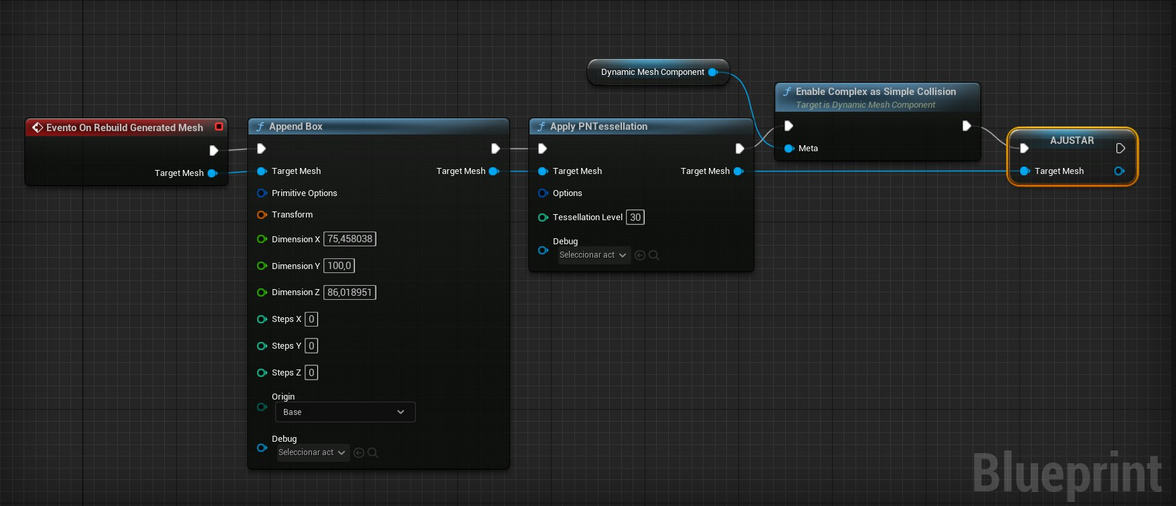
\includegraphics[width=8cm]{imagenes/bpblock}
	\caption{Blueprint de \texttt{BP\_Block}.}
	\label{fig:bpblock}
\end{figure}

\begin{figure}[H]
	\centering
	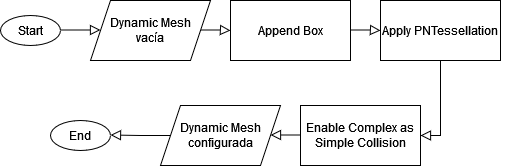
\includegraphics[width=8cm]{imagenes/flowchart1}
	\caption{Diagrama de flujo de \texttt{BP\_Block}.}
	\label{fig:fc1}
\end{figure}

El Blueprint \texttt{BP\_Block} fue el primero en implementarse, y en torno al que gira todo el proyecto. Es una clase heredada de \texttt{GeneratedDynamicMeshActor}, clase que proviene de Geometry Script y a la cual se le pueden aplicar las operaciones booleanas que necesitamos. Técnicamente, se podría usar solamente el componente \texttt{DynamicMeshComponent}, al cual también se le pueden aplicar operaciones booleanas, pero para este proyecto \textbf{es necesario usar el objeto actor} por una de sus funciones: \texttt{EventOnRebuildGeneratedMesh}. Esta función actua como un constructor en una clase convencional, pero permite, al ser posible su uso dentro de la propia Blueprint, una mayor versatilidad en la creación de la malla, además de mayor rendimiento en el editor (información extraída de la documentación oficial\footnote{\url{https://docs.unrealengine.com/5.0/en-US/geometry-script-users-guide/}}). El elemento \texttt{Target Mesh} de esta función es la malla dinámica que da forma a este actor, y sobre la que se aplican las modificaciones.

El funcionamiento de \texttt{EventOnRebuildGeneratedMesh} sigue así: primero, se le da forma con la función \texttt{AppendBox}, la cual añade una primitiva en forma de caja a la malla dinámica. Así se obtiene la forma de bloque. Una vez hecho esto, se aplica una subdivisión de triángulos usando la función \texttt{ApplyPNTessellation}. Esto es necesario para obtener un mejor rendimiento al aplicar las operaciones booleanas ya que facilita el recálculo de la topología de los triángulos. Por último, se añade colisión con la función \texttt{EnableComplexAsSimpleCollision}. Como se ha explicado previamente, normalmente las mallas de colisión son versiones simplificadas de la malla visible, pero en casos concretos se usa una malla de colisión lo más cercana posible a la visible. Unreal Engine da la posibilidad de configurar ambas, y de \textbf{usar una en lugar de la otra}. Con esta función, se usa la malla compleja en lugar de la simple, lo cual permite que, siempre que alguna herramienta colisione con el bloque, \textbf{choque siempre contra la superficie visible de este} y no contra el aire, ya que nunca se usa la versión simplificada. Una vez hecho todo esto, se aplican los cambios (\texttt{Set}) a la malla dinámica.

Originalmente, la realización de las operaciones booleanas daba lugar dentro de este Blueprint, pero un análisis posterior concluyó en que el enfoque más correcto era que se realizase dentro del código del jugador, en \texttt{VRPawn}. Por tanto, se explicará posteriormente. Destacar también que en el esquema del Blueprint se pueden apreciar líneas azules (variables) surgiendo de dos lados distintos: \texttt{Target Mesh} y \texttt{Dynamic Mesh Component}. Estas variables \textbf{son la misma}, una por referencia y la otra no, y se están usando al mismo tiempo únicamente por requerimiento de las funciones usadas, por eso no se han tenido en cuenta a la hora de diseñar el diagrama de flujo.

\section{\texttt{VRPawn}}

Este Blueprint equivale al usuario, y es donde toda su interacción con el mundo se lleva a cabo. Por tanto, es también donde se realizan todas las operaciones de las herramientas, las cuales estaban implementadas dentro de \texttt{BP\_Block} hasta cierto punto del desarrollo del martillo y cincel.

\subsection{Construcción}

\begin{figure}[H]
	\centering
	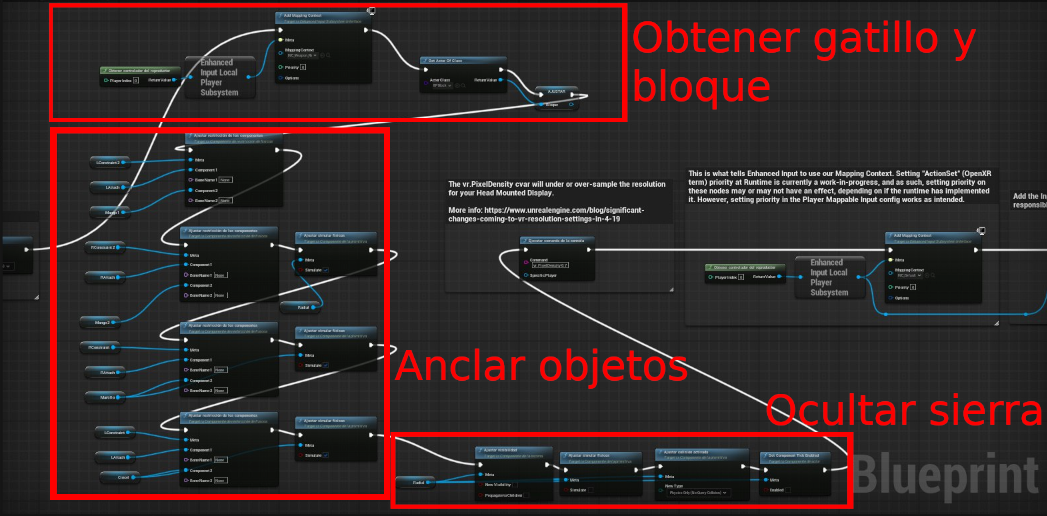
\includegraphics[width=9.2cm]{imagenes/constructor}
	\caption{\texttt{EventBeginPlay} de \texttt{VRPawn}.}
	\label{fig:constructor}
\end{figure}

\begin{figure}[H]
	\centering
	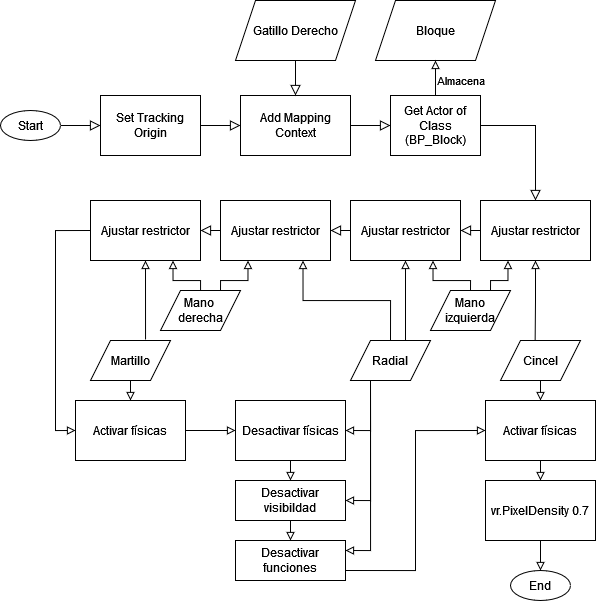
\includegraphics[width=12cm]{imagenes/flowchart2}
	\caption{Diagrama de flujo de \texttt{EventBeginPlay}.}
	\label{fig:fc2}
\end{figure}

\texttt{VRPawn} cuenta por defecto con una función llamada \texttt{EventBeginPlay}, la cual sirve para ejecutar una serie de elementos al iniciar la aplicación (como podrían ser el seguimiento de la posición del usuario o el mapeado de los controles). Por tanto, con cada nueva funcionalidad, es aquí donde deberán añadirse las partes de dicha funcionalidad que deban ejecutarse con el inicio de la aplicación.

Comentar que en este punto es también donde la plantilla modifica la variable \texttt{vr.PixelDensity}, la cual sirve para cambiar la resolución nativa de la aplicación. Para mejorar el rendimiento de la aplicación, se ha establecido dicha variable en 0.7, es decir un 70\% del valor predeterminado.

Los elementos tratados en esta función son los siguientes:

\begin{itemize}
    \item Obtener reconocimiento del gatillo derecho con \texttt{AddMappingContext} para su uso en la sierra radial.
    \item Obtener el objeto Bloque de la escena para almacenarlo como variable usando \texttt{GetActorOfClass}. Esto pasó a ser necesario al cambiar el código de las herramientas de \texttt{BP\_Block} a \texttt{VRPawn}, cambio que se hizo para un mejor manejo de las coordenadas y del cambio entre coordenadas globales y locales.
    \item Anclar todas las herramientas a los restrictores físicos. Para conseguir que las herramientas pudiesen colisionar con objetos y seguir el movimiento de las manos al mismo tiempo, se usaron \textbf{restrictores físicos}, los cuales unen dos objetos y permiten configurar diferentes parámetros sobre esta unión. De esta forma, las herramientas \textbf{siempre están en una posición natural respecto a las manos, excepto cuando un obstáculo las bloquea}. En esta función es cuando se indica qué componentes están anclados entre sí.
    \item Ocultar la sierra radial, ya que la herramienta inicial es el martillo y cincel. Para hacer esto, se desactiva su visibilidad, su colisión y sus funciones.
\end{itemize}

De esta sección cabe destacar \textbf{las dificultades enfrentadas a la hora de desarrollar las manos físicas}. Durante la investigación de cómo solucionar este problema, uno de los métodos probados fue usando la función \texttt{SetTarget LocationAndRotation}, de forma que las manos simuladas estuviesen continuamente teletransportandose a la posición de las manos reales. Esta solución, aunque útil en algunos casos, no lo es para ChiselVR, ya que únicamente sirve para dar la ilusión de choque al aplicar una fuerza leve, pero con suficiente insistencia acaba atravesando superficies sólidas. Al seguir investigando se llegó a la solución actual, en la que en lugar de teletransportarse, las manos simuladas \textbf{siguen} a las reales, chocando por el camino.

\subsection{Cincel y martillo}

\begin{figure}[H]
	\centering
	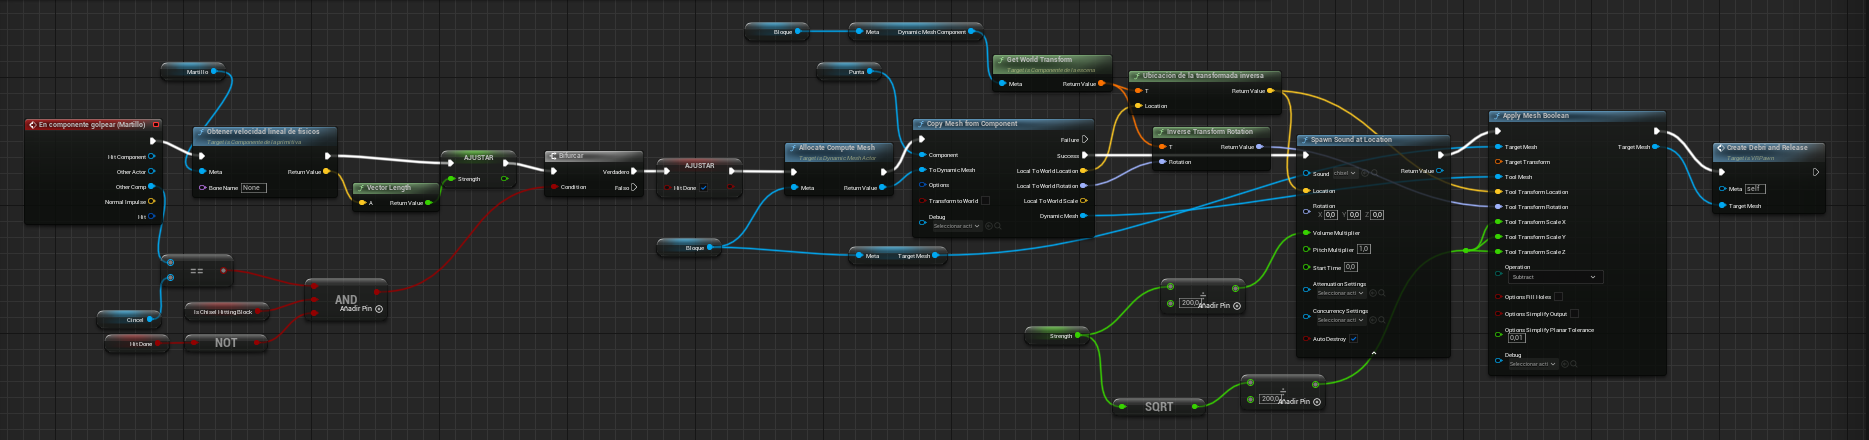
\includegraphics[width=12cm]{imagenes/martilloycincel}
	\caption{Función para cincel y martillo de \texttt{VRPawn}.}
	\label{fig:martilloycincel}
\end{figure}

\begin{figure}[H]
	\centering
	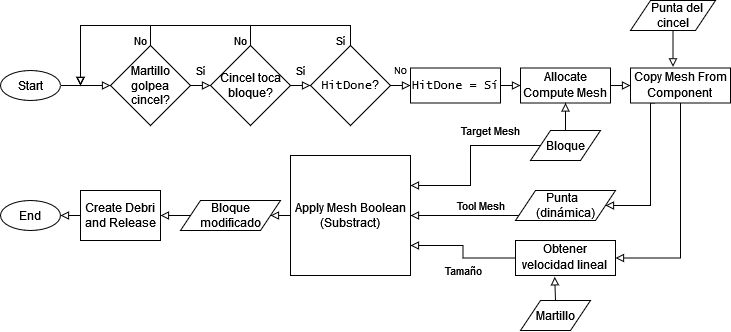
\includegraphics[width=12cm]{imagenes/flowchart3}
	\caption{Diagrama de flujo del cincel y martillo.}
	\label{fig:fc3}
\end{figure}

Esta herramienta ha sido probablemente el elemento de ChiselVR que más cambios ha tenido. Desde retoques en las colisiones a ajustes en la forma de realiza la operación booleana, el código del cincel y martillo ha pasado por diversas iteraciones para llegar a un punto en el que funcione como se esperaría. Ahora repasaremos su evolución y funcionamiento.

El primer problema a tener en cuenta es \textbf{qué se considera un golpe}. En las primeras iteraciones, un error en el funcionamiento surgía: al dar un golpe, se realizaba más de una operación. Este problema se origina en la detección de colisiones, ya que por cada \textit{tick} de la aplicación en el que tanto el bloque como el martillo estuviesen tocando el cincel, la operación se aplicaba. El movimiento humano no es lo suficientemente rápido como para realizar el golpe en un único \textit{tick}, por lo que la operación podía realizarse múltiples veces en un único golpe.

Para solucionar este problema, se crearon dos variables booleanas, \texttt{HitDone} e \texttt{IsChiselHittingBlock}, acompañadas de dos cajas de colisión en la cabeza del martillo y la punta del cincel, respectivamente. La segunda es más sencilla, simplemente cambia entre verdadero y falso dependiendo de si la caja de colisión de la punta del cincel se superpone con el bloque. La primera es algo más compleja: la variable \texttt{HitDone} empieza en falso. Cuando el martillo golpea al cincel, esta se cambia a verdadero, lo cual evita que la operación se vuelva a ejecutar de seguido con una bifurcación. Para que vuelva a estar en falso y, por tanto, se pueda realizar una nueva operación, \textbf{el cincel debe abandonar el área que compone la caja de colisiones que cubre la cabeza del martillo}. De esta forma, es necesario apartar ligeramente el martillo del cincel para volver a realizar una operación booleana, imitando así la necesidad de reunir algo de fuerza para el impacto al esculpir en la vida real (Figura \ref{fig:hitdone}).

\begin{figure}[H]
	\centering
	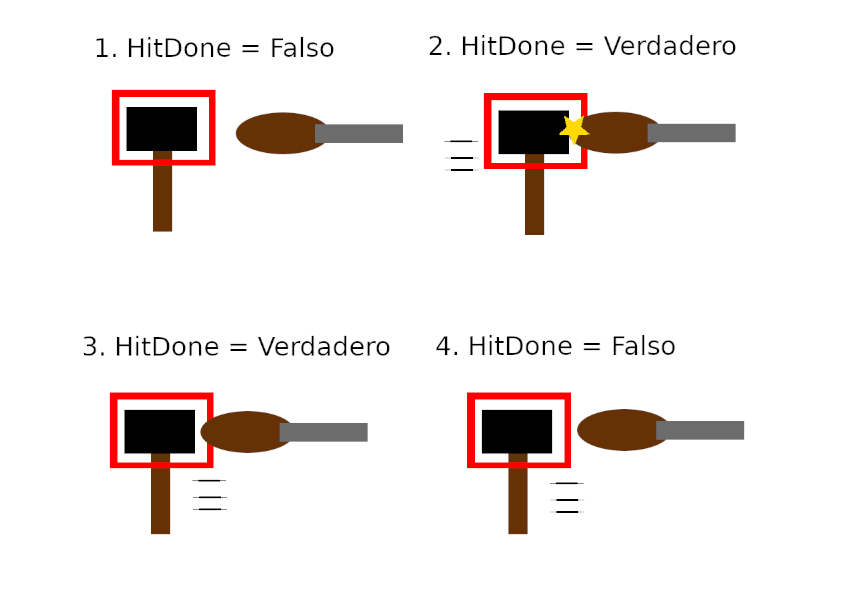
\includegraphics[width=7cm]{imagenes/hitdone}
	\caption{Esquema de la detección del golpe.}
	\label{fig:hitdone}
\end{figure}

Con este sistema, el problema de saber cuándo realizar una operación y cuándo no está solucionado. Con esto, el cálculo de la operación es más directo. Primero, se aloja una malla dinámica temporal copiando la malla de la punta del cincel, ya que las operaciones booleanas solo se pueden realizar entre mallas dinámicas. Una vez alojada, se obtiene la localización donde se realizará la operación. \textbf{La función \texttt{ApplyMeshBoolean} requiere que se le de la posición y la rotación de la herramienta en las coordenadas locales del bloque}, por lo que obtenemos las coordenadas globales de la herramienta y del bloque, y al usar la inversa de la transformación del bloque sobre la herramienta, conseguimos traducir la ubicación de esta a las coordenadas locales del bloque (Figura \ref{fig:transformacion}). Esta traducción fue costosa de alcanzar (fue una de las principales razones por la que se trasladó el código de \texttt{BP\_Block} a \texttt{VRPawn}) ya que consiste en un doble recálculo de la matriz de transformación de un objeto, lo cual requiere de \textbf{visión espacial y lógica} para realizarse correctamente, sobretodo en 3D. Con la ubicación del golpe obtenida, se aplica la operación con el tamaño dependiendo de la velocidad con la que se usase el martillo, se crean los restos si quedan trozos flotantes (se explicará el funcionamiento de esto más adelante) y se liberan todas las mallas temporales para evitar fugas de memoria.

\begin{figure}[H]
	\centering
	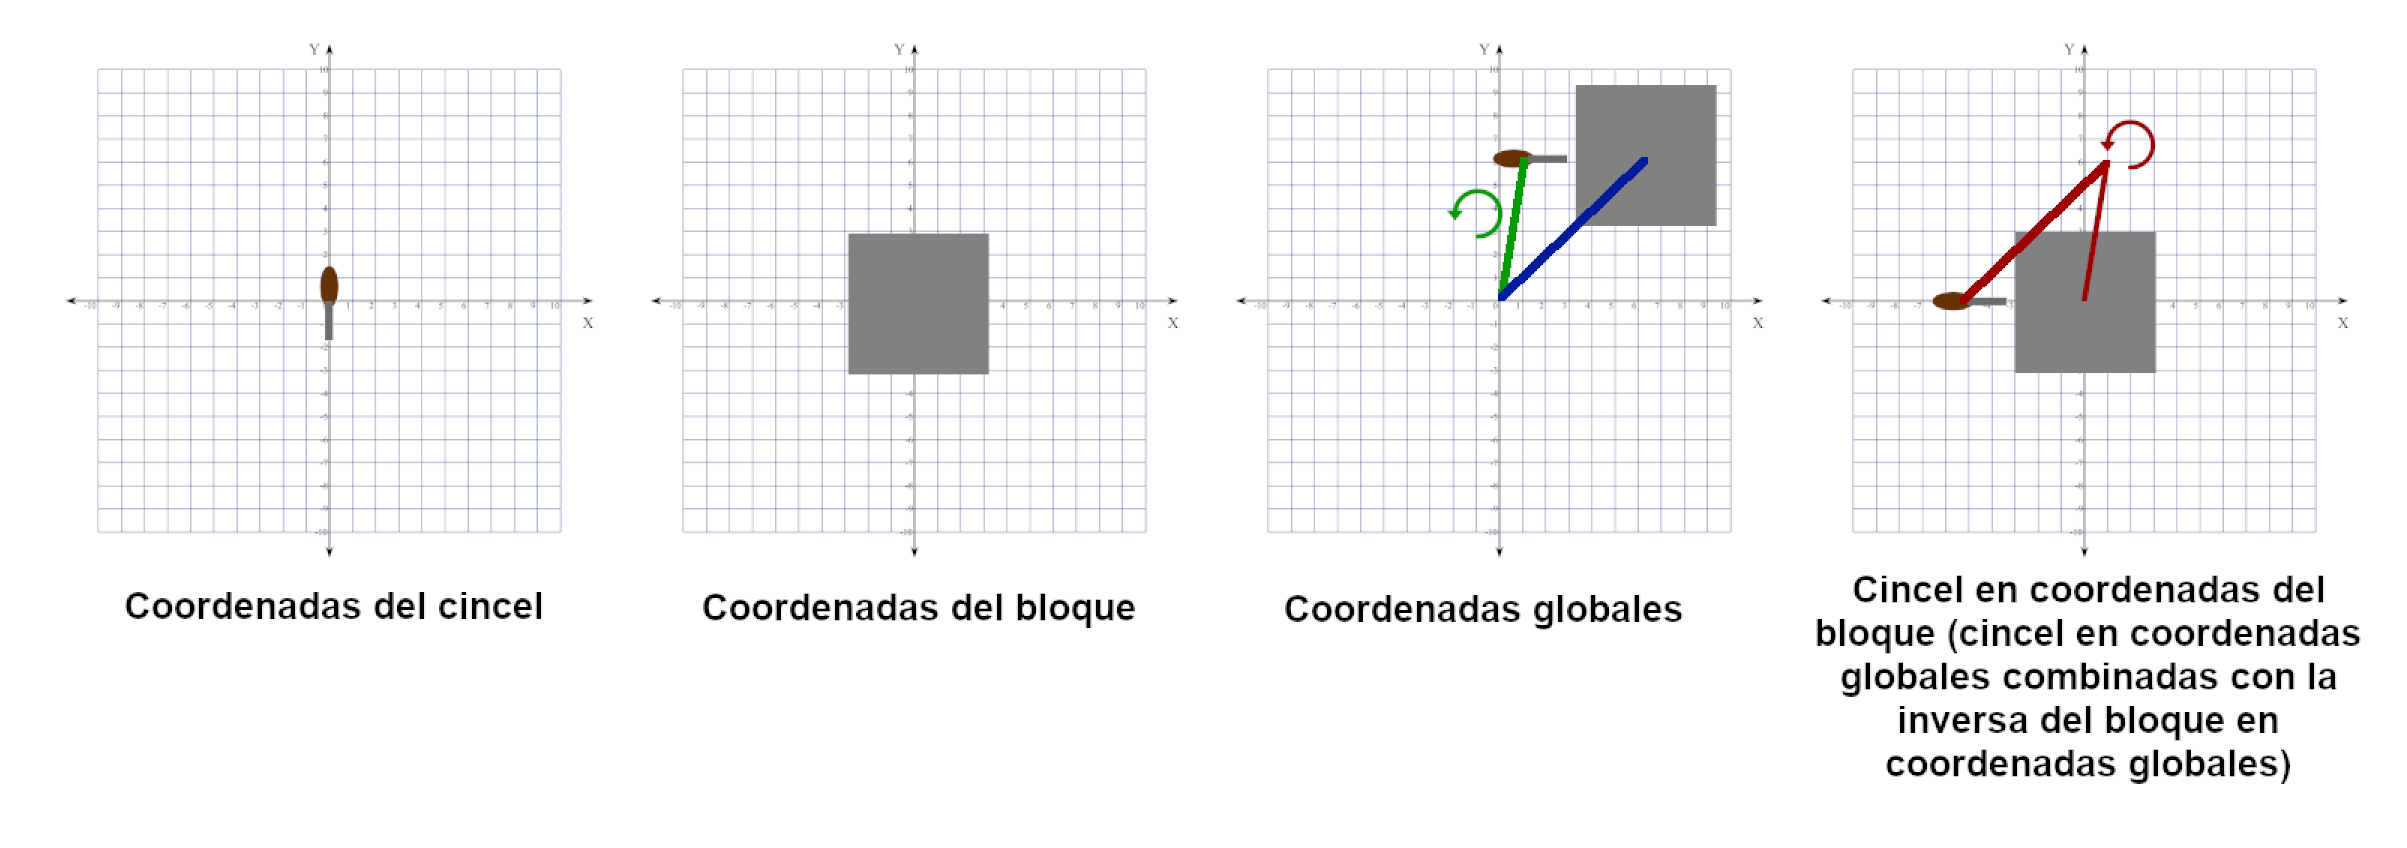
\includegraphics[width=12.5cm]{imagenes/transformacion}
	\caption{Transformación para realizar la operación booleana.}
	\label{fig:transformacion}
\end{figure}

\subsection{Sierra radial}

\begin{figure}[H]
	\centering
	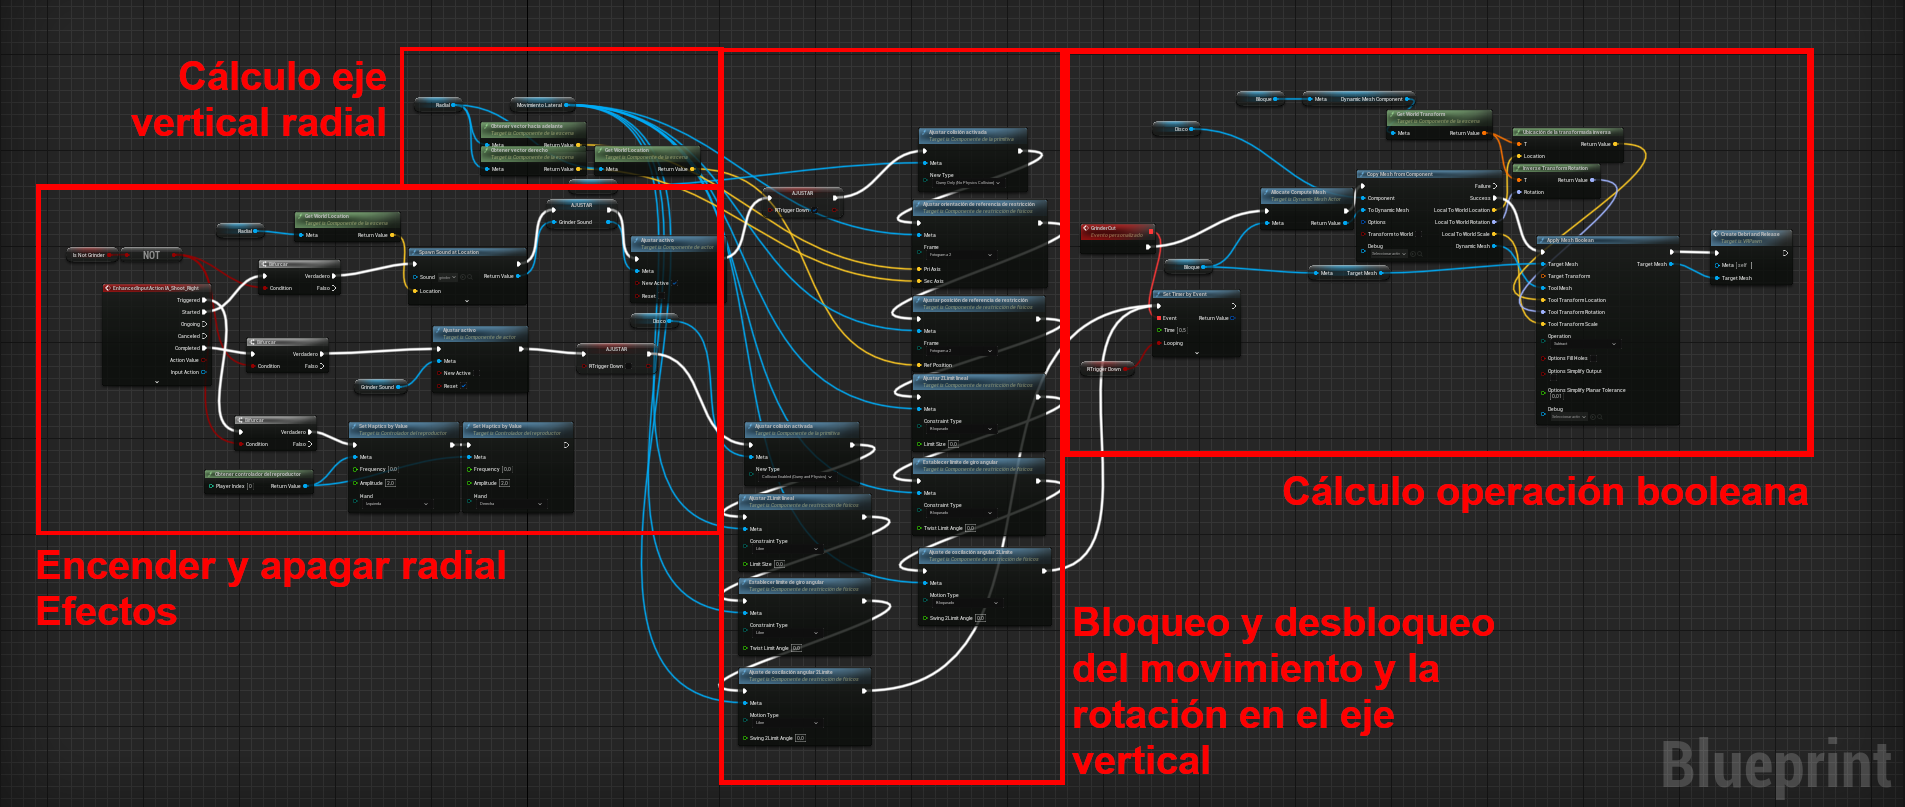
\includegraphics[width=12.5cm]{imagenes/radial}
	\caption{Función para la radial de \texttt{VRPawn}.}
	\label{fig:radial}
\end{figure}

\begin{figure}[H]
	\centering
	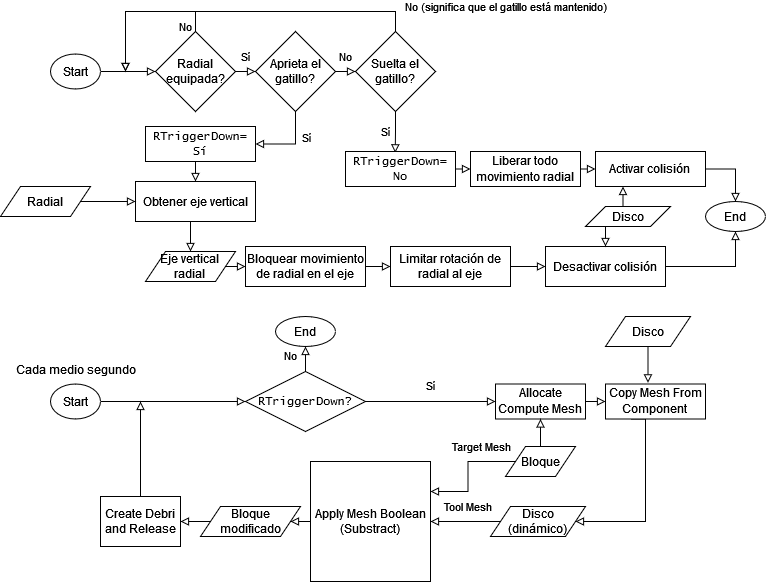
\includegraphics[width=12.2cm]{imagenes/flowchart4}
	\caption{Diagrama de flujo de la radial.}
	\label{fig:fc4}
\end{figure}

Esta herramienta hereda parte del funcionamiento del martillo y cincel, principalmente la propia realización de la operación booleana, la localización de esta y la creación de restos. Más allá de eso, tiene un funcionamiento muy distinto. En primer lugar, esta herramienta \textbf{se coge con ambas manos}, por lo que fue necesario usar prueba y error para ajustar los puntos de anclaje de las manos para que la sensación de estar sosteniendo la herramienta fuese correcta y realista. Este fue el punto más sencillo de solucionar, los siguientes provocaron más complicaciones.

Para activar la herramienta, es necesario pulsar el gatillo del mando derecho, imitando así la realidad. Con la función \texttt{EnchancedInputActionIA\_Shoot\_Right}, podemos controlar de forma precisa qué hacer dependiendo de cómo se pulse: al empezar a pulsar, cuando está mantenido, cuando se suelta, etc. Para la función de cortar material, se han usado los disparadores de \textbf{al pulsar y al soltar}. Primero, en ambos casos, se comprueba que la herramienta en uso es la sierra. Una vez comprobado, en caso de empezar a pulsar, se desactiva la colisión del disco de la sierra para que este pueda atravesar, se fija el movimiento de la herramienta a un plano paralelo a dicho disco y se activa la realización de la operación booleana con una repetición cada medio segundo. Al soltar el gatillo, se desactivan las restricciones de movimiento y la función de las operaciones, y se rehabilita la colisión del disco (Figura \ref{fig:grinder_collision}).

\begin{figure}[H]
	\centering
	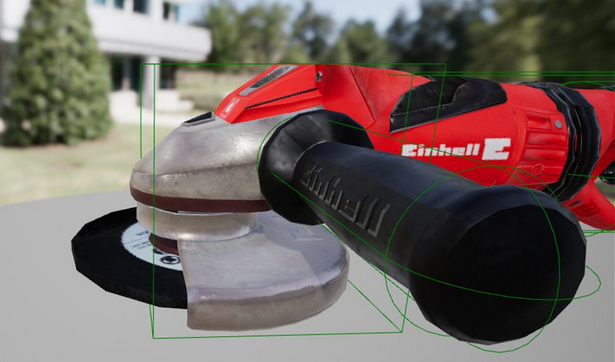
\includegraphics[width=6.3cm]{imagenes/grinder_collision}
	\caption{Malla de colisión creada para la sierra radial. La colisión del disco va aparte para que pueda chocar o no dependiendo de si está en movimiento.}
	\label{fig:grinder_collision}
\end{figure}

El factor más costoso de desarrollar para esta herramienta fue \textbf{limitar el movimiento de la sierra mientras esta está encendida}. La razón para esta limitación es evitar situaciones surrealistas al cortar el bloque: la parte que corta del disco es el borde, no la superficie, por lo que si la sierra se moviese de forma libre en todas direcciones mientras se corta no tendría sentido. Es necesario bloquear el movimiento vertical para que el corte resultante sea creíble.

Con este objetivo en mente, se abarcó el problema de distintas formas, la mayoría sin éxito. \textbf{Las formas que facilita Unreal Engine para bloquear el movimiento únicamente funcionan respecto a ejes de la escena}, por lo que el bloqueo funcionaba para mover la herramienta de forma paralela al suelo. Este obviamente no era el funcionamiento deseado, por lo que se tuvo que buscar otra forma. Finalmente, se encontraron una serie de funciones que permiten bloquear el movimiento de un objeto a partir de un plano dado, el cual se tiene que dar usando los vectores hacia delante y hacia la derecha de dicho plano. Obteniendo estos vectores de la radial y usándolos como parámetros en dichas funciones, se consiguió bloquear el movimiento en el plano deseado. Se puede ver cómo se llama a estas funciones en la parte central de la figura \ref{fig:radial}.

\subsection{Caída de escombros flotantes}

\begin{figure}[H]
	\centering
	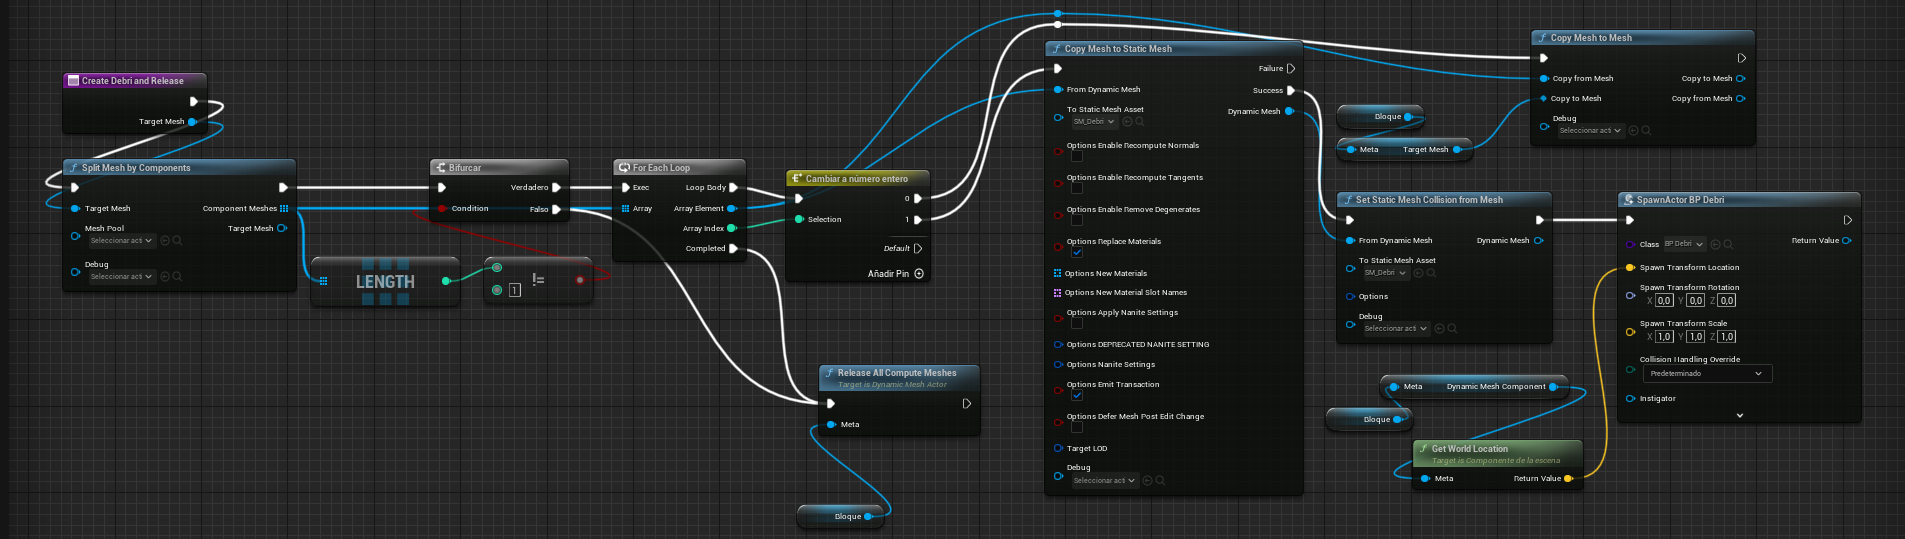
\includegraphics[width=12cm]{imagenes/createdebri}
	\caption{Función \texttt{CreateDebriAndRelease} de \texttt{VRPawn}.}
	\label{fig:createdebri}
\end{figure}

\begin{figure}[H]
	\centering
	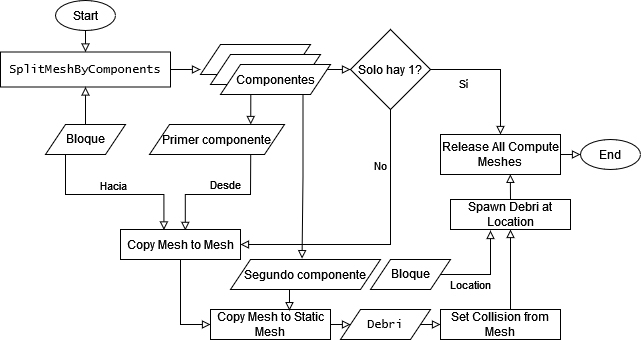
\includegraphics[width=12cm]{imagenes/flowchart5}
	\caption{Diagrama de flujo de \texttt{CreateDebriAndRelease}.}
	\label{fig:fc5}
\end{figure}

El elemento más importante a tener en cuenta respecto a efectos inmersivos fue la caída de escombros flotantes. Esto consiste en que, al realizar una operación booleana, \textbf{pueden quedar trozos inconexos del bloque principal}. Normalmente, estos trozos quedarían flotando, por lo que fue necesario implementar una forma de que cayeran al suelo.

Tras una larga investigación para ver si esto era siquiera posible, se encontró una función que nos facilita Geometry Script: \texttt{SplitMeshByComponents}. Esta función recibe una malla dinámica, detecta a través de los datos geométricos de esta todos los componentes independientes que la forman y devuelve una lista con todos estos componentes. En la documentación no se especifica cuál es el orden por defecto en el que se ordena esta lista, pero posterior experimentación concluye que es por \textbf{la altura del punto más bajo de cada componente}, siendo el primero el más bajo. Este orden nos viene perfecto, pues esto significa que el primer puesto de la lista siempre será la parte del bloque que aún está tocando el suelo y, por tanto, la que queremos que se quede.

Una vez accesibles los trozos en los que se divide el bloque, simplemente se itera sobre la lista dada: el primer objeto sustituirá al anterior bloque, de forma que este pasará a ser el mismo que antes pero sin los trozos flotantes. El siguiente trozo se guardará en un asset variable, \texttt{SM\_Debri}, el cual es el único componente del Blueprint \texttt{BP\_Debri}. Una vez guardado, se invoca un actor de la clase \texttt{BP\_Debri} en las mismas cordenadas que el propio bloque, de forma que el trozo de malla dinámica flotante es sustituido por una instancia de \texttt{BP\_Debri}, la cual tiene una cuenta atrás de autodestrucción de 5 segundos para ahorrar recursos. Una vez invocada, se le aplican colisiones simples y físicas, de forma que \textbf{cae al suelo de forma realista} (Figura \ref{fig:debri}).

\begin{figure}[H]
	\centering
	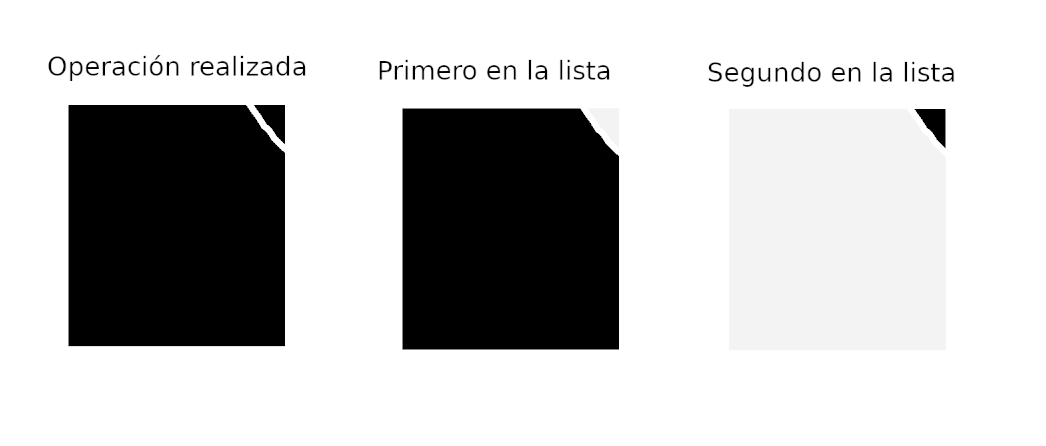
\includegraphics[width=8cm]{imagenes/debri}
	\caption{Resultado de la separación por componentes. Tanto el bloque original como los resultantes comparten exactamente las mismas coordenadas.}
	\label{fig:debri}
\end{figure}

Se podría dar la ocasión de que hubiesen más de un escombro resultante de una operación, pero por la rareza de este caso y lo pesado que podría ser computacionalmente, se ha ignorado.

Una vez hecho todo esto, se acaba la iteración por la lista. Esta función, junto a la liberación de mallas temporales para evitar fugas de memoria, están recogidos dentro de la función \texttt{CreateDebriAndRelease}, la cual se creó ya que todas las herramientas comparten este funcionamiento al final de sus respectivos códigos.

\subsection{Efectos de sonido y hápticos}

Añadir que en \texttt{VRPawn} es también donde se incluyen los diferentes efectos añadidos para la inmersión. En el caso del \textbf{martillo y cincel}, se reproduce una vibración y un sonido al mismo tiempo que se realiza la operación booleana, los cuales también varían dependiendo de la \textbf{velocidad del martillo}. En el caso de la \textbf{sierra radial}, un efecto de sonido empieza \textbf{al presionar el gatillo}, y se lanza una petición al mezclador de sonido para pararlo y reiniciarlo cuando el gatillo se suelta. Para la vibración, se mantiene una vibración constante todo el tiempo que se mantenga el gatillo pulsado.

\section{\texttt{WidgetMenu}}

Otro de los blueprints ya implementado por la plantilla es \texttt{WidgetMenu}, el cual ofrece una base para construir tu propio menú de opciones. ChiselVR contiene un total de cinco opciones las cuales funcionan así:

\begin{itemize}
    \item \textbf{Reiniciar}. Se llama a la función \texttt{OpenLevel} y se carga la misma escena.
    \item \textbf{Salir}. Se llama a la función \texttt{QuitGame}.
    \item \textbf{Cambiar mano}. Con la función \texttt{GetActorOfClass(VRPawn)} se obtiene al usuario, se comprueba el estado de la variable \texttt{HandsChanged} y, dependiendo de su estado, se ajusta para que cada mano obtenga sus datos de movimiento de un mando distinto. Al principio, se intentó cambiar físicamente la herramienta de una mano a otra, pero de esta otra forma se simplifica el código y se mantiene dentro de \texttt{WidgetMenu}. Esta función está desactivada cuando se tiene la sierra radial en las manos, pues esta solo tiene una forma de uso (Figuras \ref{fig:changedominant} y \ref{fig:fc6}).
    \item \textbf{Cincel y Martillo}. Con la función \texttt{GetActorOfClass(VRPawn)} se obtiene al usuario y se reactivan la visibilidad, físicas, colisiones y funciones de su martillo y cincel, a la vez que se teletransportan a sus manos. También se desactivan estos campos de la sierra radial, se indica con una variable booleana que la sierra radial no está activada y, en caso de que la variable \texttt{HandsChanged} esté en verdadero, se invierten las manos. Esto se debe a que, al equipar la sierra radial, las manos se ajustan a su estado original de forma automática (Figuras \ref{fig:cambiaracincel} y \ref{fig:fc7}).
    \item \textbf{Radial}. Con la función \texttt{GetActorOfClass(VRPawn)} se obtiene al usuario y se reactivan la visibilidad, físicas, colisiones y funciones de su sierra radial, a la vez que se teletransporta a sus manos. También se desactivan estos campos del martillo y cincel, se indica con una variable booleana que la sierra radial está activada y se ajustan las manos a su estado original, sea cual sea el estado de la variable \texttt{HandsChanged} (Figuras \ref{fig:cambiararadial} y \ref{fig:fc8}).
\end{itemize}

\begin{figure}[H]
	\centering
	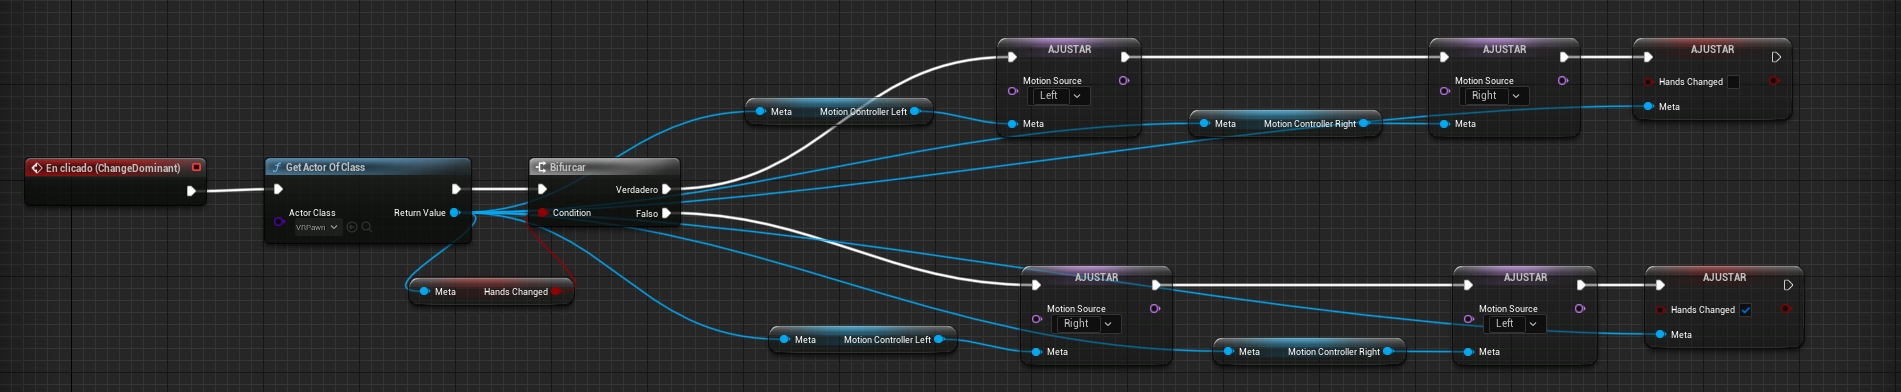
\includegraphics[width=12cm]{imagenes/changedominant}
	\caption{Función de cambio de mano en \texttt{WidgetMenu}.}
	\label{fig:changedominant}
\end{figure}

\begin{figure}[H]
	\centering
	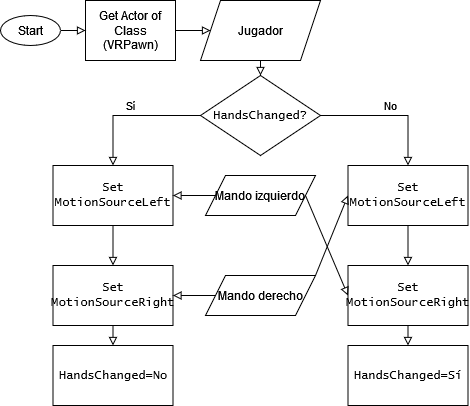
\includegraphics[width=12cm]{imagenes/flowchart6}
	\caption{Diagrama de flujo de la función de cambio de mano.}
	\label{fig:fc6}
\end{figure}

\begin{figure}[H]
	\centering
	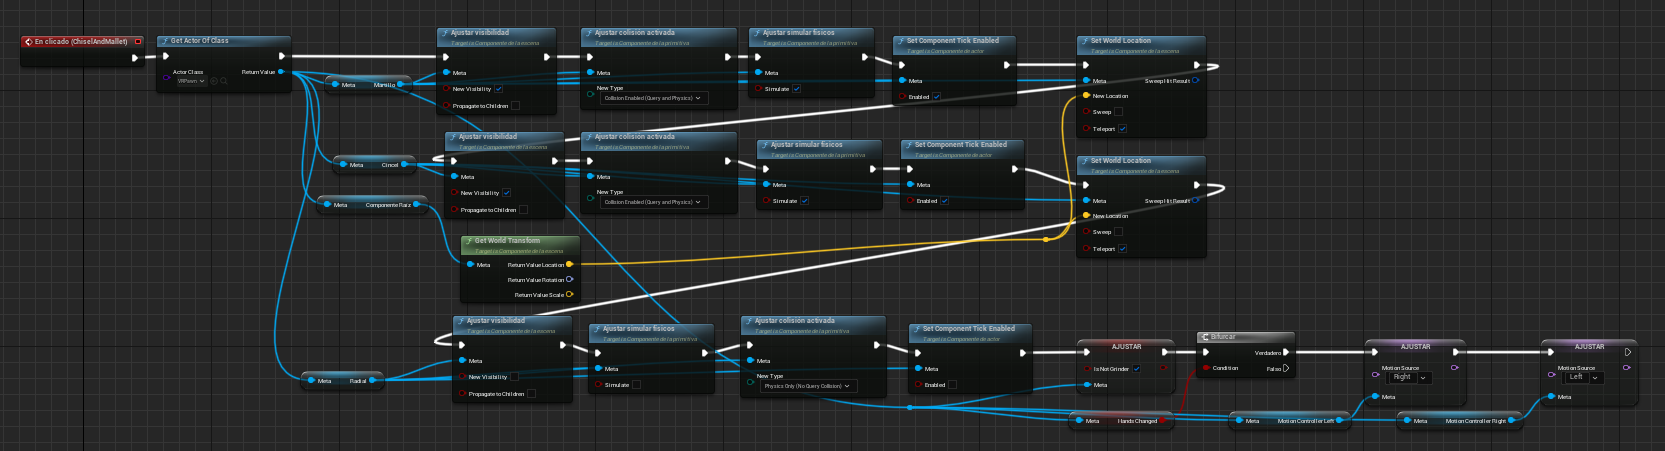
\includegraphics[width=12cm]{imagenes/cambiaracincel}
	\caption{Función de cambio a cincel y martillo en \texttt{WidgetMenu}.}
	\label{fig:cambiaracincel}
\end{figure}

\begin{figure}[H]
	\centering
	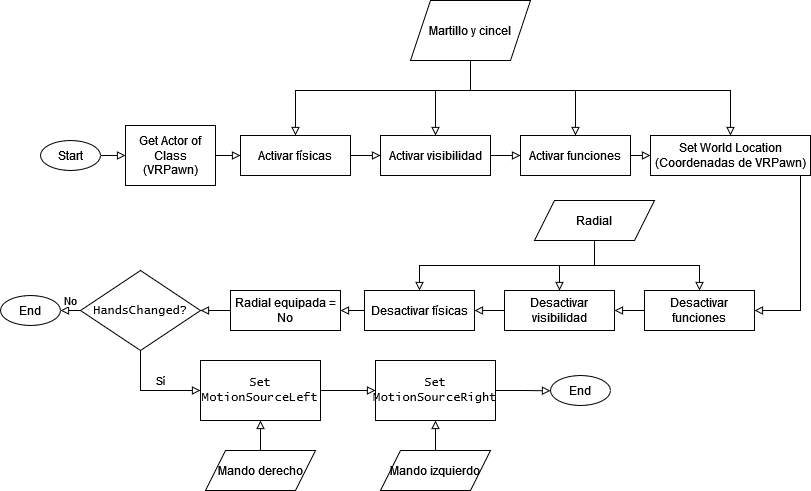
\includegraphics[width=12cm]{imagenes/flowchart7}
	\caption{Diagrama de flujo de la función de cambio a cincel y martillo.}
	\label{fig:fc7}
\end{figure}

\begin{figure}[H]
	\centering
	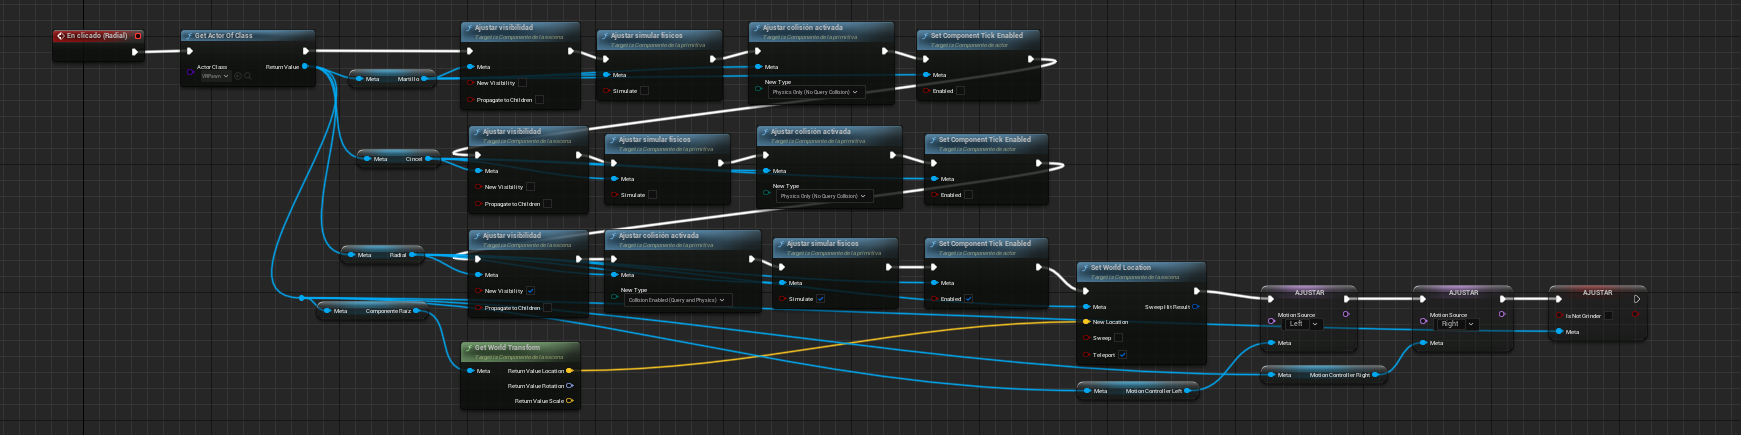
\includegraphics[width=12cm]{imagenes/cambiararadial}
	\caption{Función de cambio a radial en \texttt{WidgetMenu}.}
	\label{fig:cambiararadial}
\end{figure}

\begin{figure}[H]
	\centering
	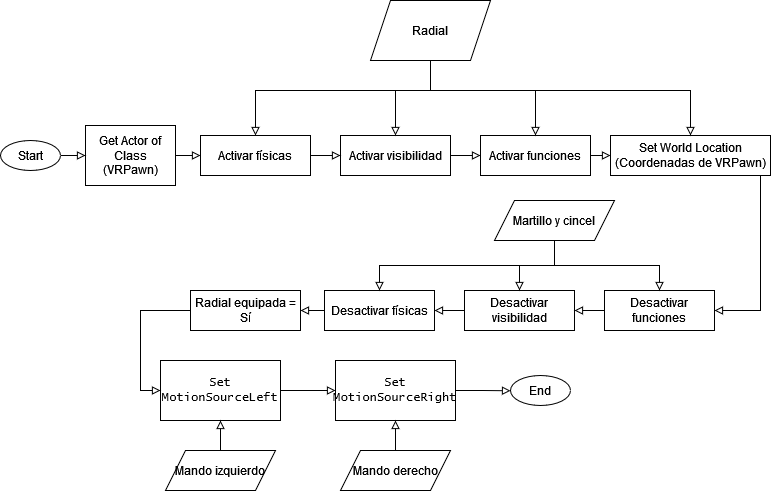
\includegraphics[width=12cm]{imagenes/flowchart8}
	\caption{Diagrama de flujo de la función de cambio a radial.}
	\label{fig:fc8}
\end{figure}

\begin{figure}[H]
	\centering
	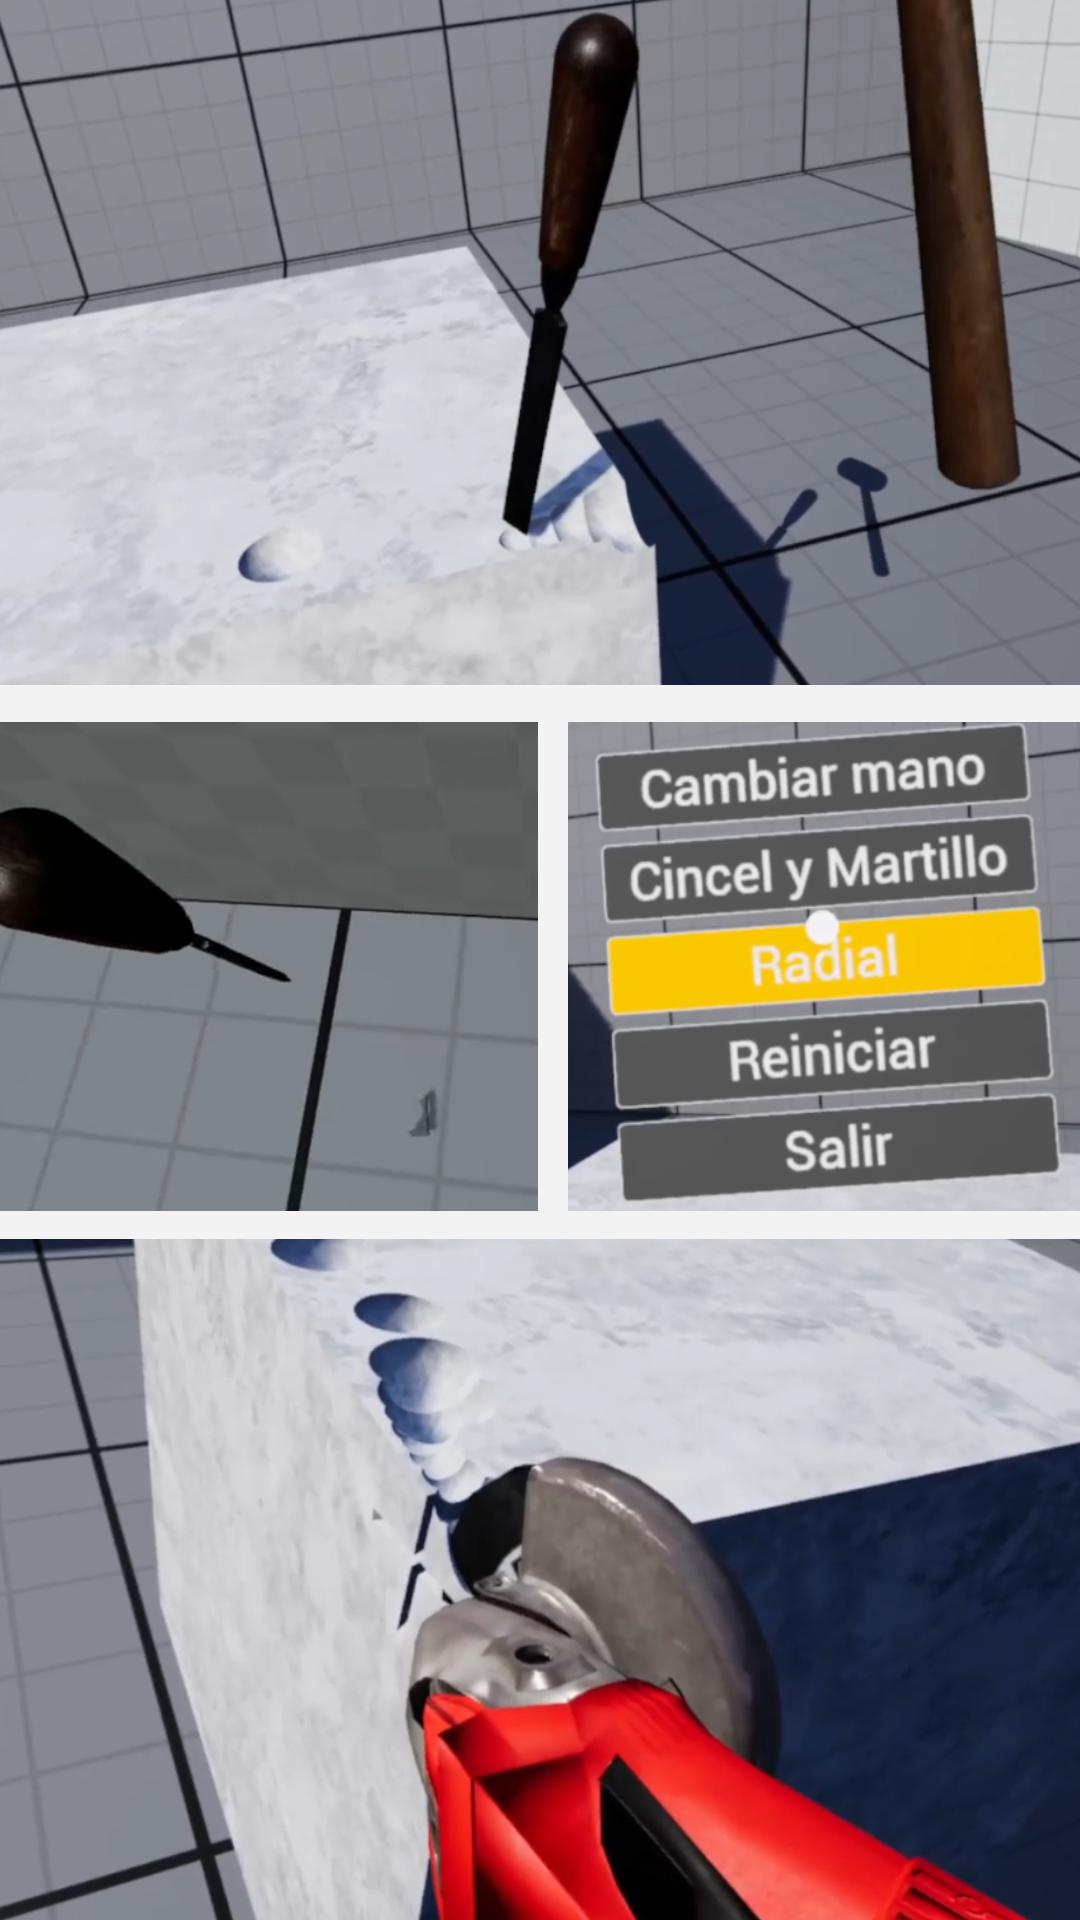
\includegraphics[width=11cm]{imagenes/screenshots}
	\caption{Capturas de pantalla de ChiselVR en ejecución.}
	\label{fig:screenshots}
\end{figure}